\section{Audição}

\begin{frame}[allowframebreaks]
  \frametitle{Som}

  Som é uma onda acústica gerada por vibração e que se propaga por um meio de transmissão (líquido, sólido ou gasoso).

  A faixa percebida pelos seres humanos é aproximadamente de 20Hz a 20kHz. Fora desta faixa
  as ondas sonoras são chamadas de infrassom e ultrassom.

  Características perceptivas:
  \begin{itemize}
  \item volume (intensidade percebida, \textit{loudness})
  \item altura (\textit{pitch})
  \item duração 
  \item timbre
  \end{itemize}

\end{frame}

\begin{frame}[allowframebreaks]
  \frametitle{Nível de pressão sonora SPL}
  O nível de pressão sonora (SPL, \textit{Sound Pressure Level}) é uma medida logarítmica 
  da pressão sonora efetiva de um som em relação a um valor de referência. A medida é em decibéis (dB)
  acima do nível de referência:
  \begin{equation}
  L_p=10 \log_{10}\left(\frac{{p_{\mathrm{{rms}}}}^2}{{p_{\mathrm{ref}}}^2}\right) =20 \log_{10}\left(\frac{p_{\mathrm{rms}}}{p_{\mathrm{ref}}}\right)\mbox{ dB} ,
  \end{equation}
  onde $p_{\mathrm{ref}}$ é a referência e $p_{\mathrm{rms}}$ é a pressão rms do som que desejamos aferir.
  Utiliza-se usualmente $p_{\mathrm{ref}} = 20 \mu Pa$ (rms) que é considerado o limiar da audição.

  \framebreak

  \begin{table}[h]
  \caption{Níveis de pressão sonora comuns em dB SPL.}\label{tab-spl}
  \begin{tabular}{ll}
  sons                     & dB SPL  \\ \hline
  turbina jato             & 150     \\
  limiar da dor            & 135     \\
  trompete                 & 130     \\
  risco de perda auditiva  & 120     \\
  britadeira               & 100     \\
  tráfego intenso          & 80 a 90 \\
  dano com longa exposição & 85      \\
  televisão                & 60      \\
  conversação              & 40 a 60 \\
  sala em silêncio         & 20 a 30 \\
  respiração calma         & 10     
  \end{tabular}
  \end{table}
\end{frame}


\begin{frame}[allowframebreaks]
  \frametitle{Nível de audibilidade}
  \vspace{-4ex}
  \begin{figure}[h]
  \centering
  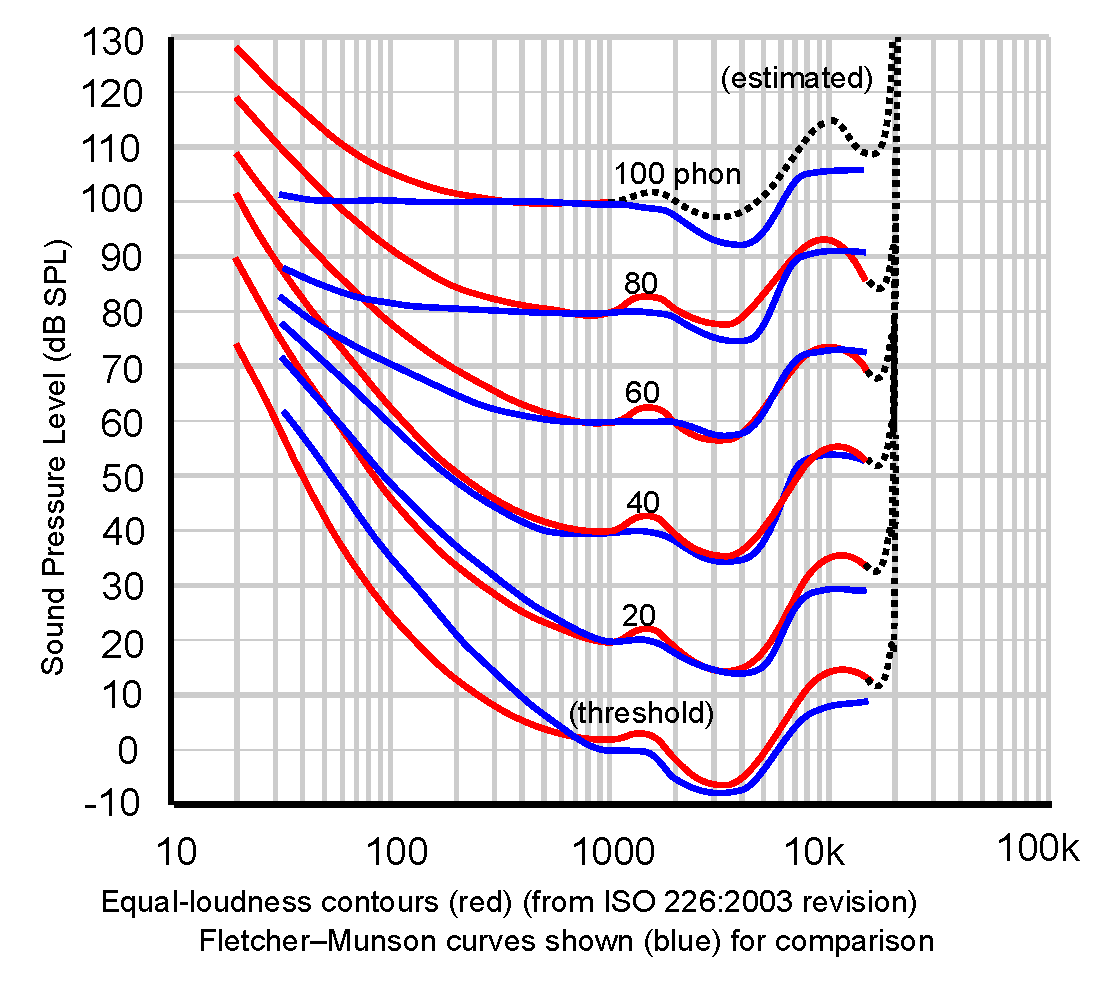
\includegraphics[width=0.45\textwidth]{images/fetchermunson.pdf}
  \caption{Curvas isofônicas (Wikipedia).}
  \label{fig-fetchermunson}
  \end{figure}
\end{frame}

\begin{frame}[allowframebreaks]
  \frametitle{Mascaramento em frequência}
  \begin{figure}[h]
  \centering
  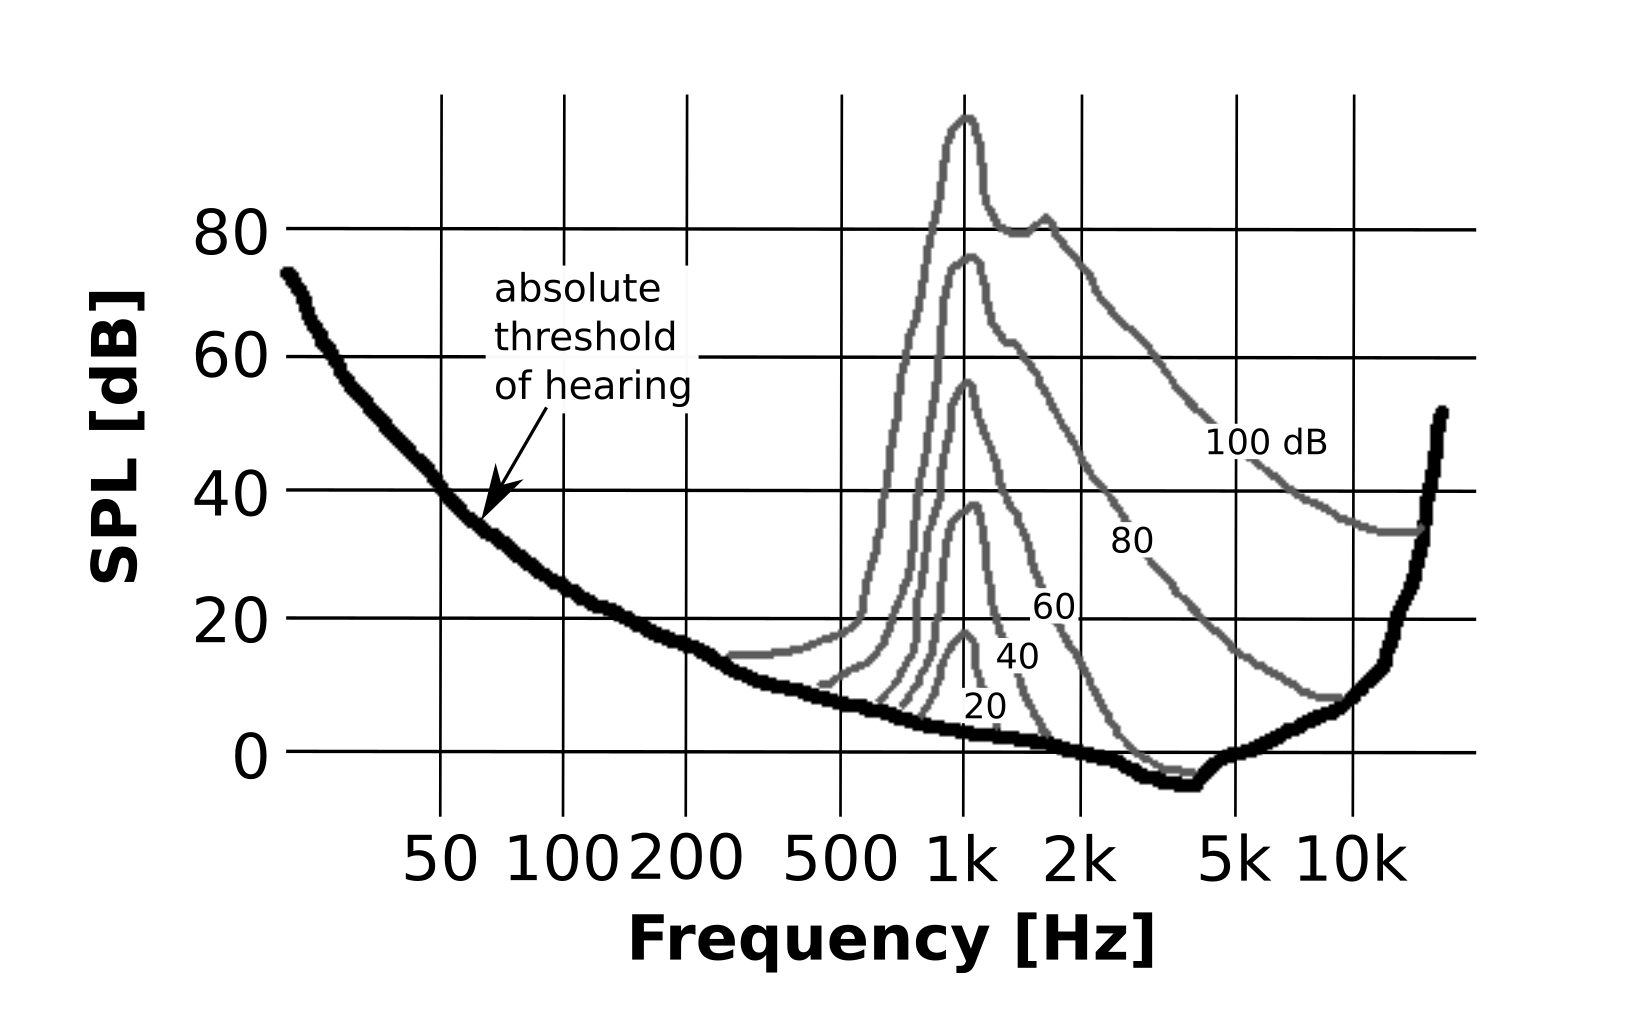
\includegraphics[width=0.6\textwidth]{images/masking.png}
  \caption{Mascaramento em frequência (Wikipedia).}
  \label{fig-masking}
  \end{figure}
\end{frame}

\begin{frame}[allowframebreaks]
  \frametitle{Mascaramento temporal}
  \begin{figure}[h]
  \centering
  
\includegraphics[width=0.65\textwidth]{images/timemasking.png}
  \caption{Mascaramento temporal (Wikipedia).}
  \label{fig-timemasking}
  \end{figure}
\end{frame}


\begin{frame}[allowframebreaks]
  \frametitle{Extensão dos instrumentos musicais}

  \begin{figure}[h]
  \centering
  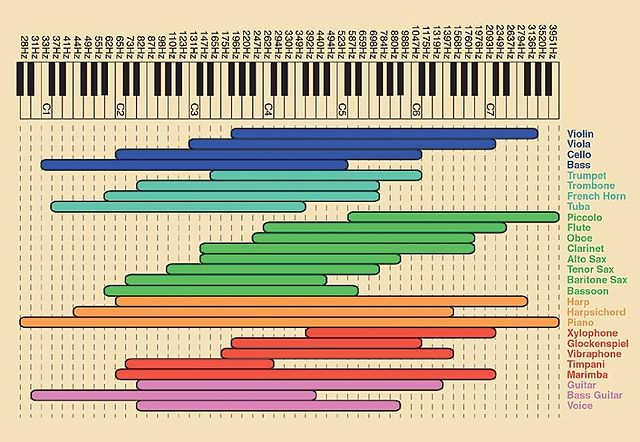
\includegraphics[width=0.55\textwidth]{images/strumenti-musicale.jpg}
  \caption{Extensão dos instrumentos musicais.}
  \label{fig-strumenti-musicale}
  \end{figure}

\end{frame}

\begin{frame}[allowframebreaks]
  \frametitle{Escala mel}
  \begin{figure}[h]
  \centering
  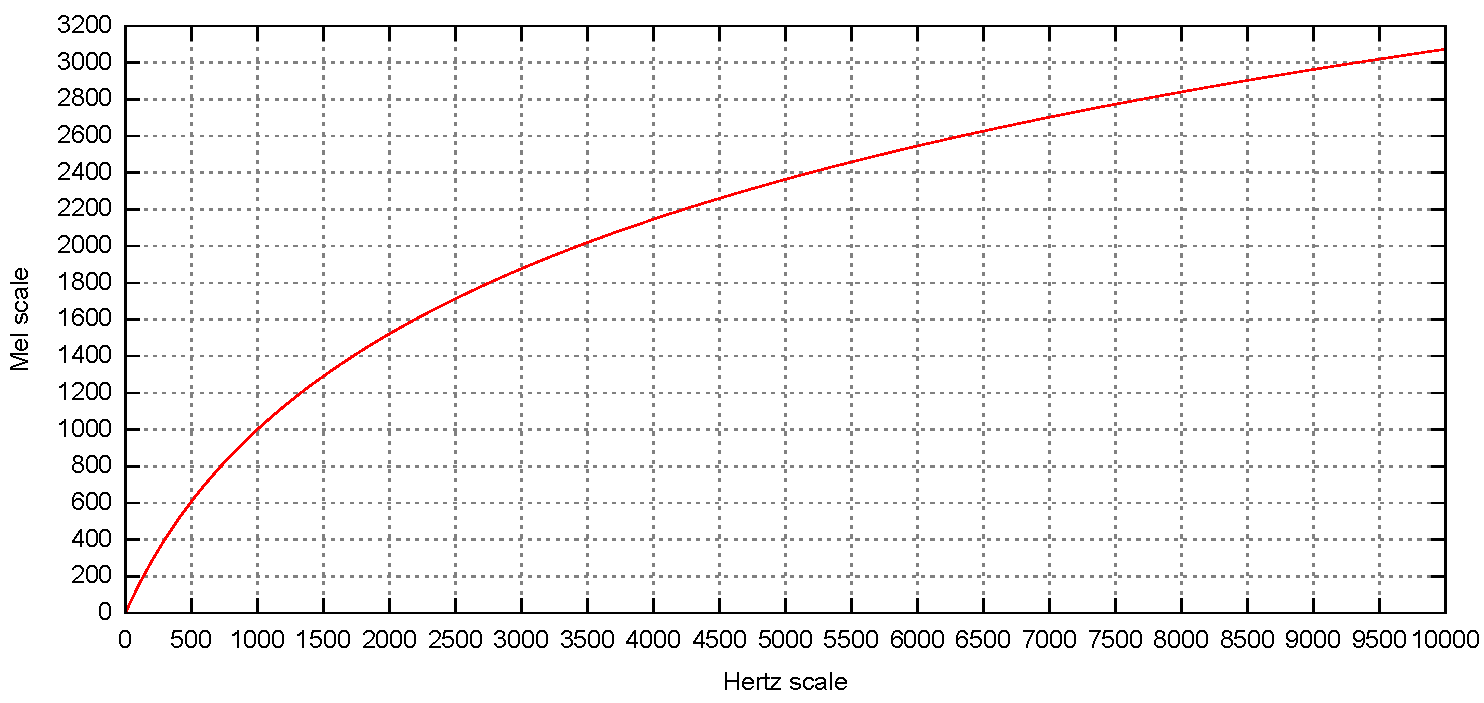
\includegraphics[width=0.6\textwidth]{images/melscale.pdf}
  \caption{Relação da escala de altura em Mel com a frequência em Hertz (Wikipedia).}
  \label{fig-mel-scale}
  \end{figure}

  \begin{equation}
  m = 2595 \log_{10}\left(1 + \frac{f}{700}\right)
  \end{equation}
\end{frame}

\begin{frame}[allowframebreaks]
  \frametitle{Banda crítica}
  \begin{figure}[h]
  \centering
  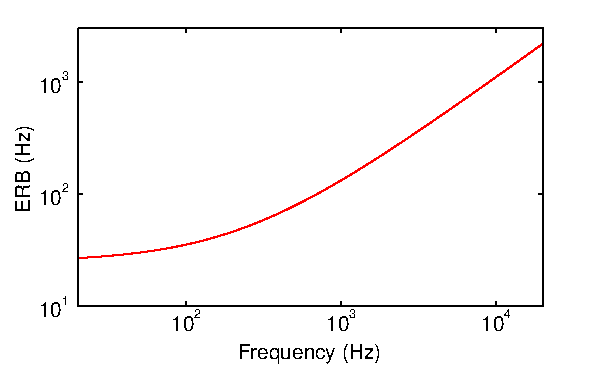
\includegraphics[width=0.6\textwidth]{images/criticalband.pdf}
  \caption{Relação da largura da banca crítica com a frequência (Wikipedia).}
  \label{fig-critical-band}
  \end{figure}
\end{frame}

\begin{frame}[allowframebreaks]
  \frametitle{Estrutura do ouvido}

  \begin{figure}[h]
  \centering
  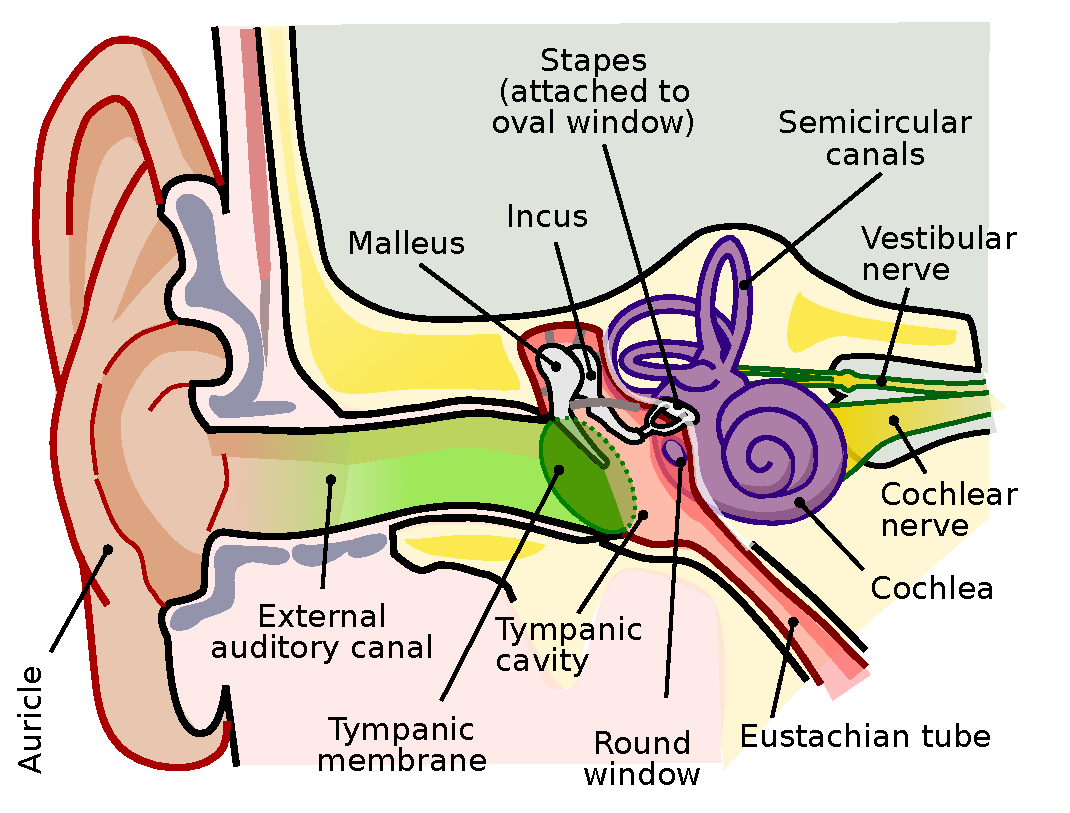
\includegraphics[width=0.5\textwidth]{images/humanear.pdf}
  \caption{Anatomia do ouvido (Wikipedia).}
  \label{fig-humanear}
  \end{figure}

  \framebreak

  \begin{figure}[h]
  \centering
  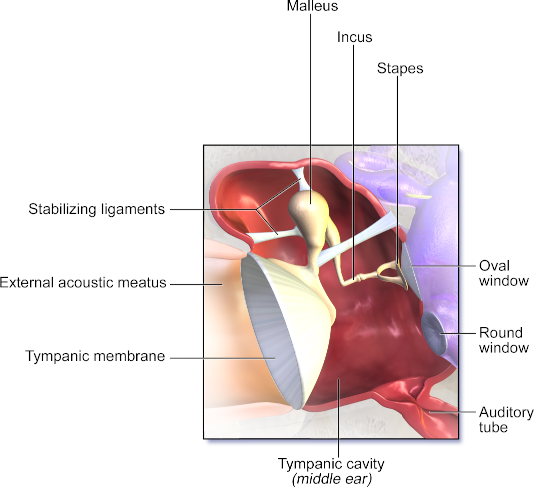
\includegraphics[width=0.4\textwidth]{images/middleear.png}
  \caption{Ouvido médio e ossículos (Wikipedia).}
  \label{fig-middleear}
  \end{figure}

  \framebreak

  \begin{figure}[h]
  \centering
  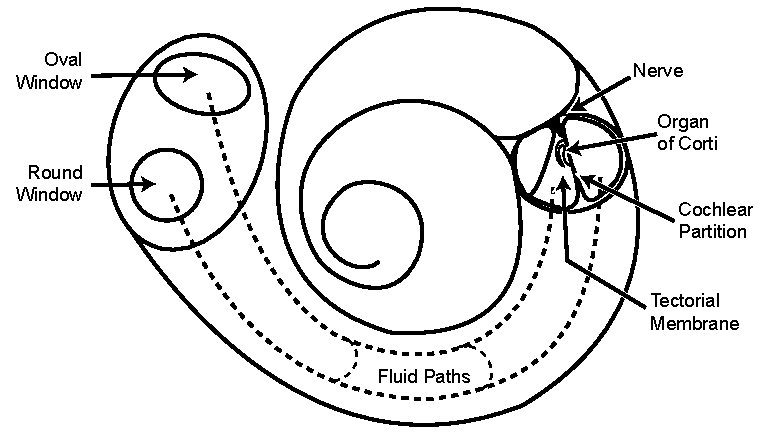
\includegraphics[width=0.5\textwidth]{images/cochlea.pdf}
  \caption{Cóclea (Wikipedia).}
  \label{fig-cochlea}
  \end{figure}

  \framebreak

  \begin{figure}[h]
  \centering
  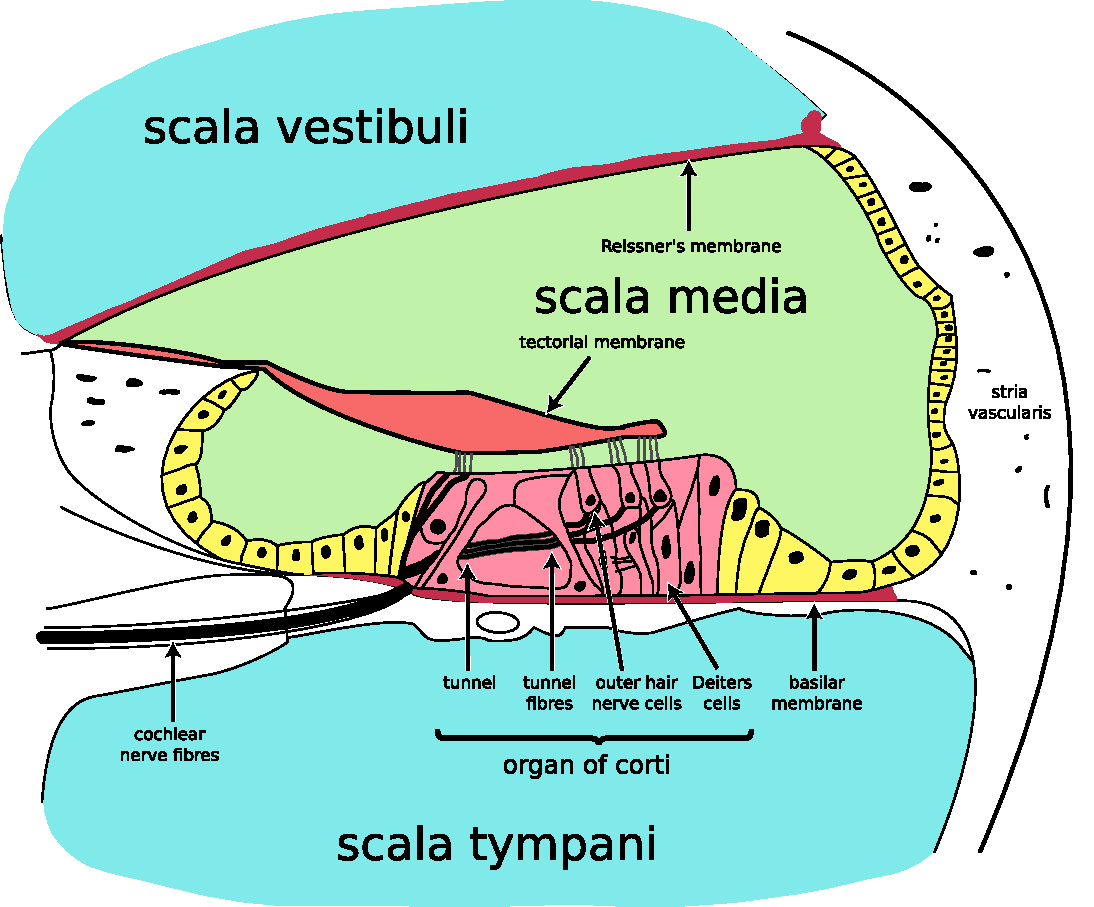
\includegraphics[width=0.5\textwidth]{images/cochlea-crosssection.pdf}
  \caption{Corte da cóclea (Wikipedia).}
  \label{fig-cochlea-crosssection}
  \end{figure}

  \framebreak

  \begin{figure}[h]
  \centering
  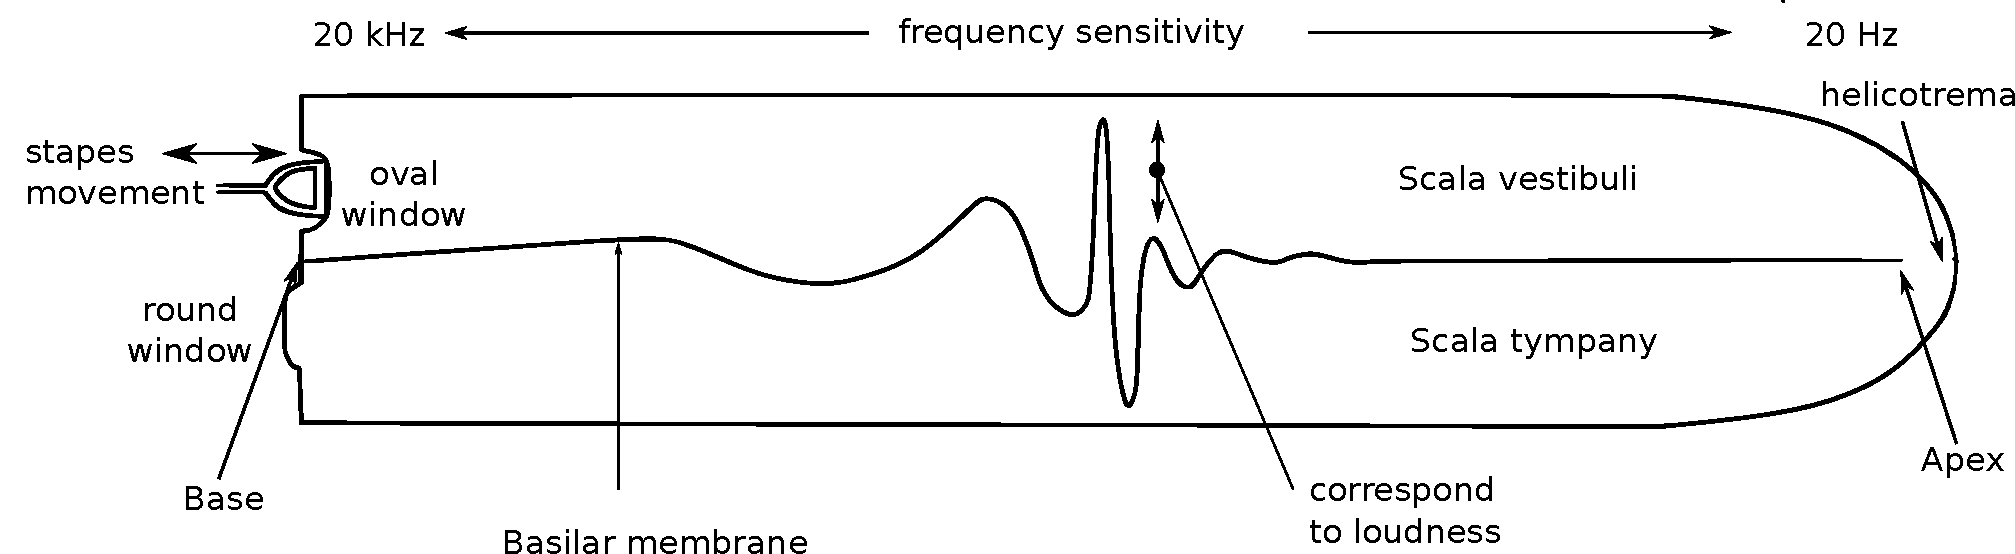
\includegraphics[width=0.75\textwidth]{images/uncoiled-cochlea.pdf}
  \caption{Cóclea (Wikipedia).}
  \label{fig-uncoiled-cochlea}
  \end{figure}

  \framebreak

  \begin{figure}[h]
  \centering
  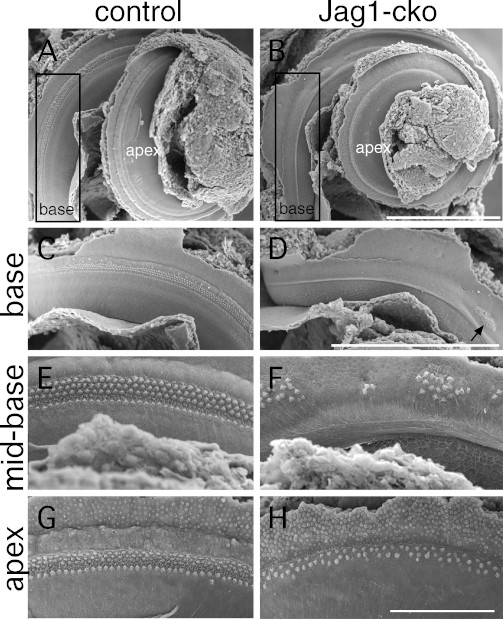
\includegraphics[width=0.3\textwidth]{images/hair-cell-pattern.jpg}
  \caption{Células ciliadas (Wikipedia).}
  \label{fig-hair-cell-pattern}
  \end{figure}

  \framebreak

  \begin{figure}[h]
  \centering
  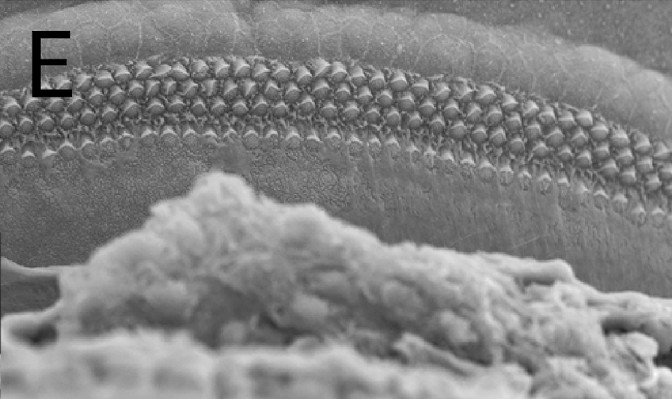
\includegraphics[width=0.65\textwidth]{images/hair-cell-pattern-E.jpg}
  \caption{Células ciliadas (Wikipedia).}
  \label{fig-hair-cell-pattern-E}
  \end{figure}

  \framebreak
  \vspace{-2ex}
  \begin{figure}[h]
  \centering
  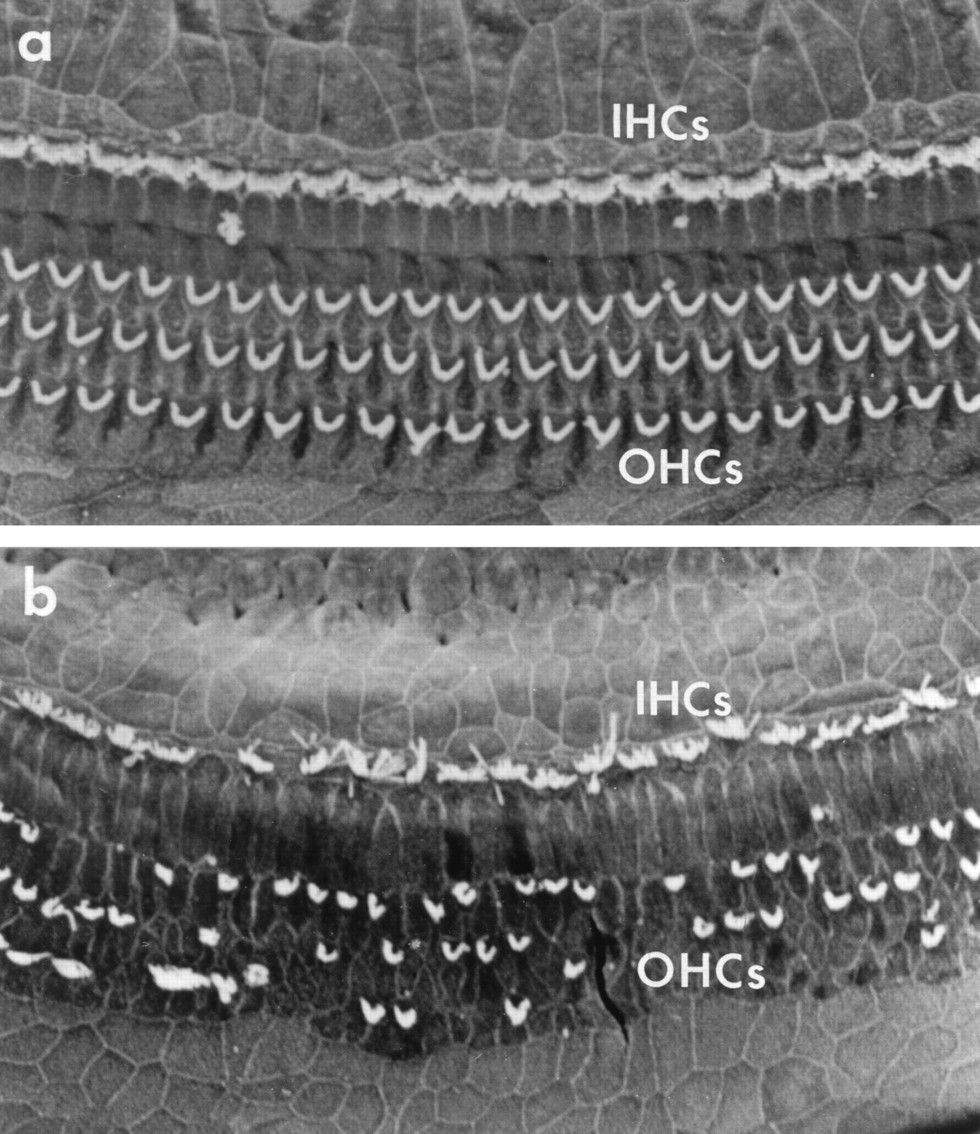
\includegraphics[width=0.35\textwidth]{images/hearingloss.jpg}
  \caption{Perda auditiva (Elizabeth M. Keithley, publicado em DOI 10.1073/pnas.97.13.6939).}
  \label{fig-hearingloss}
  \end{figure}

\end{frame}

\begin{frame}[allowframebreaks]
  \frametitle{Vídeos}
  
  
\includegraphics[width=0.35\textwidth]{images/qrcode-khanacademy-hearing.pdf}
  \url{https://www.khanacademy.org/science/health-and-medicine/nervous-system-and-sensory-infor/sound-audition-topic/v/auditory-structure-part-1}

  \framebreak 
  \begin{itemize}
  \item \url{https://www.youtube.com/watch?v=LkGOGzpbrCk}
  \item \url{https://www.youtube.com/watch?v=kzo45hWXRWU}
  \item \url{https://www.youtube.com/watch?v=w40XcUP5KrI}
  \item \url{https://www.youtube.com/watch?v=yDiXQl7grPQ}
  \item \url{https://www.youtube.com/watch?v=G-lN8vWm3m0}
  \item \url{https://www.youtube.com/watch?v=u9VMfdG873E}
  \item \url{https://www.youtube.com/watch?v=LVWTQcZbLgY}
  \end{itemize}

  \framebreak

  \vspace{-3ex}
  
\includegraphics[width=0.35\textwidth]{images/qrcode-kandel.pdf}

  \vspace{-2ex}
  \bibentry{kandel2014}
  
  \url{https://books.google.com.br/books?id=cq1_BAAAQBAJ&pg=PA391}
\end{frame}
